\tikzstyle{startstop} = [rectangle, rounded corners, minimum width=3cm, minimum height=1cm,text centered, draw=black, fill=red!30]
\tikzstyle{io} = [trapezium, trapezium left angle=70, trapezium right angle=110, minimum width=3cm, minimum height=1cm, text centered, draw=black, fill=blue!30]
\tikzstyle{process} = [rectangle, minimum width=3cm, minimum height=1cm, text centered, draw=black, fill=orange!30]
\tikzstyle{decision} = [diamond, minimum width=3cm, minimum height=1cm, text centered, draw=black, fill=green!30]
\usetikzlibrary{shapes.geometric}
\tikzstyle{database} = [cylinder, minimum width=3cm, minimum height=1cm, text centered, draw=black, fill=yellow!30, shape border rotate=90, aspect=0.25]

\chapter{Atomic Pair Distribution Function: \\Theory and Computation}
\section{Theory}
To properly understand the PDF and its limitations we need to derive its mathematics.
The following derivation has been performed numerous times but most recently and completely by Farrow and Billinge, it is reproduced here for clarity and completeness.
\subsection{Derivation}
\section{Theory}
To properly understand the PDF and its limitations we need to derive its mathematics.
The PDF has been previously derived many times so it is not re-derived here.
This discussion of the PDF and its gradients use the notation of Farrow and Billinge. \cite{Farrow2009}
\subsection{Derivation}
Many of the above techniques require the gradient of the PES.
This in turn requires the gradient of the PDF to be derived.
Mathematically treating thermal vibrations will also be discussed in this section.
Systems which are truly extended materials, like powders with particle sizes larger than 10nm, are best formulated as systems with periodic boundaries.
Thus, the equations for a periodically bound PDF need to be developed as well, with their gradients.
\subsection{Analytically Gradients}
Many optimization algorithms and simulations methodologies, including HMC, require not only the potential energy of a given configuration but also the forces acting on that configuration.
These forces are described by the gradient of potential energy of the system which in turn requires the gradient of the PDF.
As previously shown the PDF is the Fourier Transform of the Debye equation.
Since the Fourier Transform is expressed as an integral we can exchange the order of the gradient and the integral, allowing us to calculate the analytical gradient of the Debye equation and FFT the resulting function.
The Debye equation, with a Debye-Waller vibrational correction is
\begin{equation}
F(Q) = \frac{1}{N \langle f \rangle^{2}} \sum_{j\neq i} f_i^{*}(Q)f_j(Q) \exp(-\frac{1}{2}\sigma_{ij}^{2}Q^{2}) \frac{\sin(Qr_{ij})}{r_{ij}}
\end{equation}
where
\begin{eqnarray}
  \sigma_{ij}^{2} = (\vec{u}_{ij} * \hat{d}_{ij})^{2}\\
  \vec{u}_{ij} = \vec{u}_{i} - \vec{u}_{j}\\
  \hat{d}_{ij} = \frac{\vec{d}_{ij}}{r_{ij}}\\
  r_{ij} = ||\vec{d}_{ij}|| \\
  \vec{d}_{ij} =
  \begin{bmatrix}
    q_{ix} - q_{jx}\\
    q_{iy} - q_{jy} \\
    q_{iz} - q_{jz}
  \end{bmatrix}
\end{eqnarray}
where $Q$ is the scatter vector, $f_i$ is atomic scattering factor of the $i$th atom, and $r_{ij}$ is the distance between atoms $i$ and $j$ and has $q$ dependence. \cite{Jeong2002}
For simplicity's sake we will break up $F(Q)$ so that
\begin{equation}
F(Q) = \alpha \sum_{j\neq i} \beta_{ij} \uptau_{ij} \Omega_{ij} \label{eq:abto}
\end{equation}
where
\begin{eqnarray}
  \alpha = \frac{1}{N \langle f \rangle^{2}} \label{eq:alpha} \\
  \beta_{ij} = f_i^{*}(Q)f_j(Q)\label{eq:beta}\\
  \uptau_{ij} = \exp(-\frac{1}{2}\sigma_{ij}^{2}Q^{2}) \label{eq:tau}\\
  \Omega_{ij} = \frac{\sin(Qr_{ij})}{r_{ij}} \label{eq:omega}
\end{eqnarray}

\noindent The derivatives are as follows:
\begin{equation}
\frac{\partial}{\partial q_{i,w}} F{ (Q )} = \alpha \sum_{j} \beta_{ij} (\frac{\partial \uptau_{ij}}{\partial q_{i,w}}  \Omega_{ij} + \uptau_{ij} \frac{\partial \Omega_{ij}}{\partial q_{i,w}}) \label{eq:grad_fq}
\end{equation}
where
\begin{eqnarray}
  \frac{\partial \Omega_{ij}}{\partial q_{i,w}}  = \frac{Q\cos(Qr_{ij}) - \Omega_{ij}}{r_{ij}^{2}} (q_{i,w}-q_{j,w})\\
  \frac{\partial \uptau_{ij}}{\partial q_{i,w}} = \frac{\sigma_{ij}Q^{2} \uptau_{ij}}{r_{ij}^{3}}   ((q_{i,w} - q_{j,w}) \sigma_{ij}- ( u_{i,w} - u_{j,w})r_{ij}^{2})
\end{eqnarray}

Since $\vec{u}_{ij}$ is a variable as well, we need the derivative with respect to it as well.
Thus
\begin{eqnarray}
\frac{\partial}{\partial u_{i,w}} F{ (Q )} = \alpha \sum_{j} \beta_{ij} \frac{\partial \uptau_{ij}}{\partial u_{i,w}}  \Omega_{ij}\\
\frac{\partial \uptau_{ij}}{\partial u_{i,w}} = - \frac{\sigma_{ij}Q^{2} \uptau_{ij}}{r_{ij}}  (q_{i,w} - q_{j,w})
\end{eqnarray}
\subsubsection{Without ADPs}
Without ADPs the equations simplify down to
\begin{equation}
F(Q) = \frac{1}{N \langle f \rangle^{2}} \sum_{j\neq} f_i^{*}(Q)f_j(Q) \frac{\sin(Qr_{ij})}{r_{ij}}
\end{equation}
and
 \begin{equation}
\frac{\partial}{\partial q_{i,w}} F{ (Q )} = \alpha \sum_{j} \beta_{ij} \frac{\partial \Omega_{ij}}{\partial q_{i,w}}
\end{equation}
use of these equations, when ADPs are not appropriate (like at cryogenic temperatures), greatly speeds up the computation.

\subsubsection{Periodic Boundary Conditions}
Periodic boundary conditions can be helpful when simulating extended solids or large nanoparticles. In this case all the non-crystallinity is contained within the simulation box and the box is repeated to create the longer distance peaks observed in the PDF. To perform this we can break up the Debye equation into two main parts, the part that describes the interatomic distances within the simulation box and those between boxes. Neglecting the thermal motion portion:
\begin{equation}
  F(Q) = \frac{1}{N \langle f \rangle^{2}}(\sum_{j\neq i} f_i^{*}(Q)f_j(Q) \frac{\sin(Qr_{ij})}{r_{ij}} + \sum_{i,j} f_i^{*}(Q)f_j(Q) \frac{\sin(QR_{ij})}{R_{ij}})
\end{equation}
where
\begin{eqnarray}
  R = |\vec{r} + \vec{\nu}|\\
  \vec{\nu} = \gamma_1*\vec{a} + \gamma_2*\vec{b} + \gamma_3*\vec{c}
\end{eqnarray}
where $\gamma_{i}$ is the number of copies of the simulation box in the $i$th direction, and $\vec{a}, \vec{b}, \vec{c}$ are the lattice or superlattice directions.

%This can be represented in the form of equation \ref{eq:abto} with ADPs as:
\begin{equation}
F(Q) = \alpha(\sum_{j\neq i}  \beta_{ij} \uptau_{ij} \Omega_{ij} + \sum_{i,j}  \beta_{ij} \zeta_{ij} \eta_{ij}) \label{eq:adp_pbc}
\end{equation}
where:
\begin{eqnarray}
    \zeta_{ij} = \exp(-\frac{1}{2}\varsigma_{ij}^{2}Q^{2}) \label{eq:zeta}\\
    \eta_{ij} = \frac{\sin(QR_{ij})}{R_{ij}} \label{eq:eta}\\
    \varsigma_{ij}^{2} = (\vec{u}_{ij} * \hat{D}_{ij})^{2}\\
    \hat{D}_{ij} = \frac{\vec{D}_{ij}}{R_{ij}}\\
    \vec{D}_{ij} = \vec{r} + \vec{\nu}
\end{eqnarray}
The additive nature of the first and second term of equation \ref{eq:adp_pbc} implies that we can separate the gradient.
Thus the gradient is:
\frac{\partial}{\partial q_{i,w}} F{ (Q )} = \alpha (\sum_{i!=j} \beta_{ij} (\frac{\partial \uptau_{ij}}{\partial q_{i,w}}  \Omega_{ij} + \uptau_{ij} \frac{\partial \Omega_{ij}}{\partial q_{i,w}}) + \sum_{i,j} \beta_{ij} (\frac{\partial \uptau_{ij}}{\partial q_{i,w}}  \Omega_{ij} + \uptau_{ij} \frac{\partial \Omega_{ij}}{\partial q_{i,w}})) \label{eq:pbc_grad_fq}
The first term gradient will be the same as equation \ref{eq:grad_fq}.
The second term however will have its own distinct gradients:
\begin{eqnarray}
  \frac{\partial \eta_{ij}}{\partial q_{i,w}}  = \frac{Q\cos(QR_{ij}) - \eta_{ij}}{R_{ij}^{2}} (q_{i,w}-q_{j,w} + \nu_{w})\\
  \frac{\partial \zeta_{ij}}{\partial q_{i,w}} = \frac{\varsigma_{ij}Q^{2} \eta_{ij}}{R_{ij}^{3}}   ((q_{i,w} - q_{j,w} +\nu_{w}) \varsigma_{ij}- (u_{i,w} - u_{j,w})R_{ij}^{2})\\
\end{eqnarray}
\begin{eqnarray}
\frac{\partial}{\partial u_{i,w}} F{ (Q )} = \alpha \sum_{j} \beta_{ij} \frac{\partial \uptau_{ij}}{\partial u_{i,w}}  \Omega_{ij}\\
\frac{\partial \uptau_{ij}}{\partial u_{i,w}} = - \frac{\sigma_{ij}Q^{2} \uptau_{ij}}{r_{ij}}  (q_{i,w} - q_{j,w})
\end{eqnarray}

\todo[inline]{Also should include PBC gradients, although they are trivial, maybe?}
\todo[inline]{How does this compare against the Ewald simulation technique for ionic solutions}

\begin{equation}
\frac{1.0 \sigma_ij}{R_{ij}^{3}} Q^{2} \uptau_ij \left(R_{ij}^{2} \left(- u_{ix} + u_{jx}\right) + \left(\nu_{x} + q_{ix} - q_{jx}\right) \left(\left(u_{ix} - u_{jx}\right) \left(\nu_{x} + q_{ix} - q_{jx}\right) + \left(u_{iy} - u_{jy}\right) \left(\nu_{y} + q_{iy} - q_{jy}\right) + \left(u_{iz} - u_{jz}\right) \left(\nu_{z} + q_{iz} - q_{jz}\right)\right)\right)
\end{equation}




\section{Computation}
Simply deriving the equations for the PDF is not enough.
The many body nature of the PDF equation make analytical solution of the structure from the PDF impossible.
Thus, the PDF must be computed from a structural candidates and compared against experimental results to evaluate the relability of the model.

\subsection{HPC and GPUs}
To properly solve the structure of materials the PDF will need to be computed many times and checked against experimental results.
This requires computation of the PDF, potentialy over many atoms.
Calculating these PDFs requires a fast, highly parallized, computational framework.
\subsubsection{GPUs and Parallelization}
\begin{figure}
    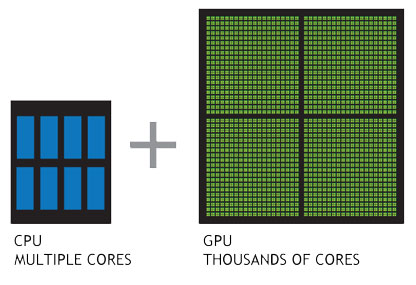
\includegraphics[width=\textwidth]{cpu-and-gpu}
    \caption{Comparison of the CPU and GPU chip architectures}
    \label{fig:cpu_vs_gpu}
\end{figure}
Computing the PDF is an embarrassingly parallel problem.
The basic procedure is to calculate the reduced structure factor $F(Q)$ for each atom pair and momentum transfer vector, sum over all the atom pairs, and Fourier transform the structure to the PDF.
The first part of this procedure is perfectly parallizable, as each atom pair is seperate from the others.
The summation over all the atomic reduced structure factors can be parallelized via distributed summing.
Lastly the FFT can be parallelized using existing parellel FFT algorithms.

GPUs are particularly well suted to the task of computing PDFs.
GPU chip architecture is designed to perform many task simultaniously by having potentially thousands of cores.

\subsubsection{Map from ij space to k space}
The above equations, although formally correct, are very ineffiecent. $F(Q)$ and its gradient are indexed over all the atoms twice, however there are symmetries that allow us to only compute over the atom pairs esentially mapping from an $n$x$n$ space, $ij$ space, to a $\frac{n(n-1)}{2}$ space, $k$ space.
For $F(Q)$ we apply the following mapping
\begin{figure}[!ht]
\begin{center}
\begin{tikzpicture}
    \node (E) at (0,0) {$E$};
    \node[right=of E] (F) {$E'$};
    \node[right=of F] (Z) {$Z$};
    \node[below=of F] (N) {$B'$};
    \node[below=of E] (M) {$B$};
    \draw[->] (E)--(F) node [midway,above] {$\psi$};
    \draw[->] (F)--(Z) node [midway,above] {$\Sigma$};
    \draw[->] (M)--(N) node [midway,below] {$\psi'$};
    \draw[->] (E)--(M) node [midway,left] {$\phi$};
    \draw[->] (N)--(Z) node [midway,left] {$\Sigma'$};
\end{tikzpicture}
\end{center}
\end{figure}
where $E$ denotes the atomic coordinates in $ij$ space, $E'$ denotes $F(Q)$ before the summation in $ij$ space, $B$ denotes the atomic pairs in $k$ space, $B'$ denotes $F(Q)$ in $k$ space, and $Z$ denotes the final summed $F(Q)$.  For the operators, $\phi$ denotes the mapping from $ij$ space to $k$ space $k = j + i * \frac{i - 1}{2}$, $\psi$ and $\psi'$ denote the $F(Q)$ operation in $ij$ and $k$ space, respectivly. $\Sigma$ denotes the sum over all the atoms.  

To properly define $\Sigma'$ we must establish whether $F(Q)$ is an even function.  
We can accomplish this by examining each of the portions of $F(Q)$, $\alpha, \beta ,\uptau, \Omega$.
$\Omega$ is even, since $r_{ij}$ is the interatomic distance, which is the same despite a flip of indicies, $Q$ does not depend on the atomic indicies, and since $Qr_{ij}$ is even so is $\sin{Qr_{ij}}$.  Thus, $\Omega$ is even.  Providing similar analysis to $\uptau$ we can see that while $\vec{u}_{ij}$ is odd, so is the unit displacement vector between the two atoms, thus the two odds cancel out.
Intuitivly this makes sense, since the $F(Q)$ equation is fundamentally interested in the interatomic distances which is even.  Thus, switching atom indicies does not change $F(Q)$.
Due to the even nature of the $F(Q)$ operator the $\Sigma'$ operator sums over all the atom pairs, and multiplies by two to reflect the double counting of the $\Sigma$ operator.

For the gradient a similar mapping is used:
\begin{figure}[h!]
\begin{center}
  \begin{tikzpicture}
    \node (E) at (0,0) {$E$};
    \node[right=of E] (F) {$E'$};
    \node[right=of F] (Z) {$Z$};
    \node[below=of F] (N) {$B'$};
    \node[below=of E] (M) {$B$};
    \draw[->] (E)--(F) node [midway,above] {$\psi$};
    \draw[->] (F)--(Z) node [midway,above] {$\Sigma$};
    \draw[->] (M)--(N) node [midway,below] {$\psi'$};
    \draw[->] (E)--(M) node [midway,left] {$\phi$};
    \draw[->] (N)--(Z) node [midway,left] {$\tilde{\phi}\Sigma$};
\end{tikzpicture}
\end{center}
\end{figure}

In this mapping, however, we use the $\tilde{\phi}\Sigma$ operator.  This operator simultaniously performs a reverse mapping from $k$ to $ij$ space, and a summation with the correct symmetry.  In this case the $\psi$ and $\psi'$ operators, which denote the $\grad{F(Q)}$ operator in $ij$ and $k$ space, are antisymmetric.  Intuitivly this makes sense as an extension of Newton's Second Law, since each particle's interation is felt oppositely by its partner.
\subsubsection{Periodic Boundary Conditions}
Periodic boundary conditions can be helpful when simulating extended solids or large nanoparticles. In this case all the non-crystallinity is contained within the simulation box and the box is repeated to create the longer distance peaks observed in the PDF. To perform this we can break up the Debye equation into two main parts, the part that describes the interatomic distances within the simulation box and those between boxes. Neglecting the thermal motion portion:
\begin{equation}
  F(Q) = \frac{1}{N \langle f \rangle^{2}}(\sum_{j\neq i} f_i^{*}(Q)f_j(Q) \frac{\sin(Qr_{ij})}{r_{ij}} + \sum_{i,j} f_i^{*}(Q)f_j(Q) \frac{\sin(QR_{ij})}{R_{ij}})
\end{equation}
where 
\begin{eqnarray}
  R = |\vec{r} + \vec{u}|\\
  \vec{u} = \gamma_1*\vec{a} + \gamma_2*\vec{b} + \gamma_3*\vec{c}
\end{eqnarray}
\section{Experiment}
PDF experiments are generally performed at synchrotron light sources, as only these sources can provide the need flux, energy, and high momentum transfer vectors needed to obtain relyable PDFs.

\section{Data Processing Workflow}
Processing the raw pixel intensities to the PDF is very important as we are extracting most of our interesting information out of very high $Q$ data.
This data relies on good statistics and sound background subtraction.
Talk about papers from Billinge Group with thin film PDF and dilute NP solutions.
Diagram of the overall data processing workflow.
Discuss the NSLS-II data stack.
\begin{figure}
\centering
\begin{tikzpicture}[thick,scale=0.6, every node/.style={scale=0.6}]
    \node (img) [startstop] at (0,0) {Image Data};
    \node [database, right=of img] (fs)  {FileStore};
    \node[startstop, below=of img] (imeta) {Image Metadata};
    \node[startstop, below=of imeta] (emeta) {Environmental Metadata};
    \node[startstop, below=of emeta] (bmeta) {Beamline Metadata};
    \node[startstop, below=of bmeta] (smeta) {Sample Metadata};
    \node[database, right=of emeta] (mds) {MetadataStore};
    \node[process, right=of mds] (db) {DataBroker};
%     \node[io, right=of db] (lfg) {Load Data};
%     \node[io, below=of lfg] (lbg) {Load Background};
%     \node[process, right=of lfg] (maskfg) {Mask Data};
%     \node[process, right=of lbg] (maskbg) {Mask Background};
%     \node[process, right=of maskfg] (ifg) {Azimuthally Integrate Data};
%     \node[process, right=of maskbg] (ibg) {Azimuthally Integrate Background};
%     \node[process, right=of ifg] (bgsubs) {Subtract Background};

%     \draw[->] (img) -- ++(0,1) -- ++($(fs)+(0,1)$)node[] -- (fs);
%     \draw[->] (F)--(Z) node [midway,above] {$\Sigma$};
%     \draw[->] (M)--(N) node [midway,below] {$\psi'$};
%     \draw[->] (E)--(M) node [midway,left] {$\phi$};
%     \draw[->] (N)--(Z) node [midway,left] {$\tilde{\phi}\Sigma$};
\end{tikzpicture}
\caption{Database Loading Workflow. Data is loaded from various sources, including images and text files, into the FileStore and MetadataStore databases. Data is then retrieved from the databases using the databroker.}
\end{figure}
\subsection{MetadataStore Side Loading}
Design of sidewinder-spec for loading the data into metadatastore.
Most of the design considerations went into the loaders, which are different for each experiment.

\subsection{Detector $Q$ resolution} \label{subsec:qres}
To properly azimuthaly integrate the images taken from the detector the $Q$ resolution of the pixels must be calculated.
Integrating using even bins will cause pixels which are not on the same ring to be binned together, causing the incorrect value of $I(Q)$ to be obtained and a larger standard deviation in the integrated data.
To properly calculate the $Q$ resolution the resolution of each of the pixels in $2\theta$ must be calculated.
\begin{figure}
    \centering
    \begin{tikzpicture}
        \draw (0,0) node[anchor=north]{$A$}
          -- (4,0) node[anchor=north]{$C$}
          -- (4,4) node[anchor=east]{$B$}
          -- cycle;
        \draw (0,0) node[anchor=north]{$A$}
          -- (4,0) node[anchor=north]{$C$}
          -- (4,6) node[anchor=south]{$B'$}
          -- cycle;
    \end{tikzpicture}
    \caption{Scattering onto a flat detector}
    \label{fig:scattering_digram}
\end{figure}
Figure \ref{fig:scattering_digram} shows the scattering of x-rays onto a flat image plate detector.
In this diagram the bottom of the $n$th pixel is $B$ while the top is $B'$.
The resolution of this pixel in $2\theta$ is $\angle BAC - \angle B'AC$.
Thus the resolution, calculated from the distances is
\begin{equation}
\Delta 2 \theta = \arctan{\frac{b}{d}} - \arctan{\frac{t}{d}}
\end{equation}
where d is the sample to detector distance, b is the distance to the bottom of a pixel, and t is the distance to the top of that pixel.
Note that these distances need to have been corrected for detector tilt and rotation.
Thus the resolution of a pixel in $Q$ is
\begin{equation}
\Delta Q = \frac{4\pi(\sin{\arctan{\frac{b}{d}}} - \sin{\arctan{\frac{t}{d}}})}{\lambda}
\end{equation}
where $\lambda$ is the x-ray wavelength.

For a Perkin Elmer image plate, like the one used at the NSLS-II's XPD and the APS's 11-ID-B, the resolution function is shown in \ref{fig:res_func}.
For the same detector the number of pixels per $Q$ is shown in \ref{fig:pixel_hist}
\begin{figure}[!ht]
  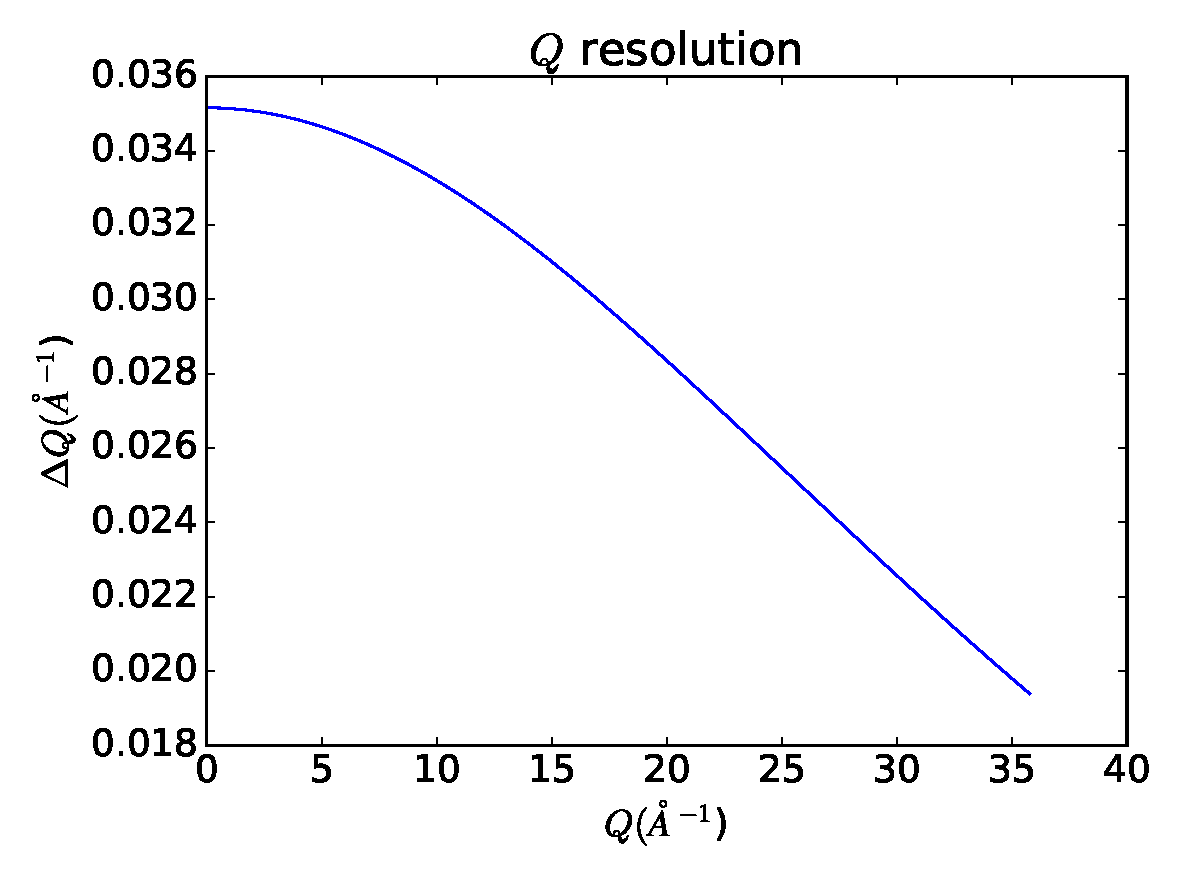
\includegraphics[width=\textwidth]{res}
\caption{$Q$ resolution as a function of $Q$.}
\label{fig:res_func}
\end{figure}

\begin{figure}[!ht]
  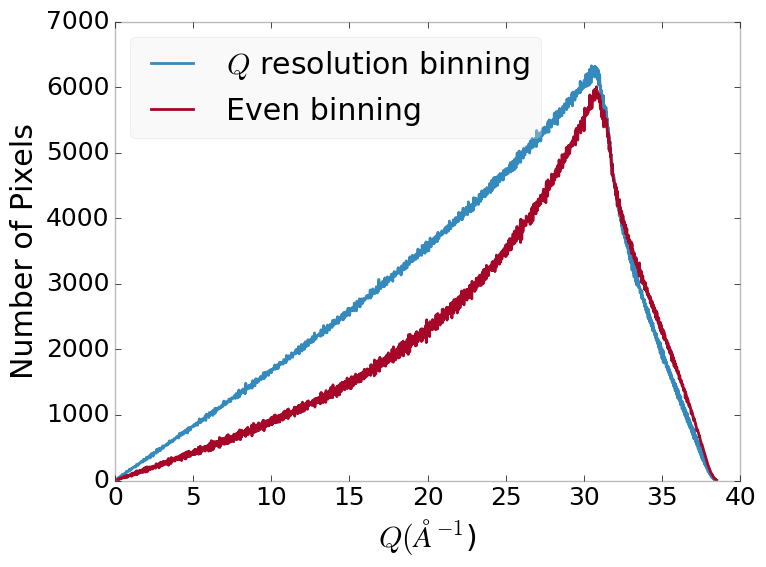
\includegraphics[width=\textwidth]{pixels}
\caption{Number of pixels as a function of $Q$, binned at the $Q$ resolution of the detector.}
\label{fig:pixel_hist}
\end{figure}

\subsubsection{Automated Mask Generation}
Detector masking is an important part of any x-ray scattering workflow as dead/hot pixels, streak errors, and beamstop associated features can be averaged into the data changing the signal and its statistical significance.
While some features, like the beamstop holder, can be easily observed and masked by hand other are much more difficult to observe even on large computer monitors.
Additionally, while dead/hot pixels and streaks are usually static the hot pixels associated with textured or single crystal scattering or cosmic rays are not.
Thus, coming up with an automated method for finding such erroneous pixels is important, especially as high flux diffraction beamlines can generate data very quickly.

While this problem can be quite complex in the most general case, we can use the annular symmetry of the powder scattering pattern to our advantage, by comparing a pixel against pixels in the same ring.
Since non-textured powder scattering should produce the same pixel intensity for a given ring we can mask any pixels which are $\alpha$ standard deviations away from the mean.
This method relies on the aforementioned pixel binning algorithm, as using miss sized bins will cause some pixels which should be in separate rings to be put together, and others which should be in the same ring to be separated.
In that case the masking algorithm will overestimate the number of pixels to be masked due to the additional statistical variation in the sample.

The masking algorithm procedure takes in the image and a description of the pixel positions in either distance from the point of incidence or in $Q$.
The image is then integrated twice, producing both the mean $I(Q)$ and the standard deviation of each $I(Q)$ ring.
The mask is created by comparing the pixel values against each ring's standard deviation and theshold $\alpha$.
Note that the theshold can be a funciton of distance from the point of incidence or $Q$.

To study the effectiveness of the masking we ran the algorithm against both simulated experimental data.
In the case of the simulated data four systems were created:
1) dead/hot pixels with varying numbers of defective pixels,
2) beamstop holder vith varying beamstop holder transmittance,
3) rotated beamstop holder vith varying beamstop holder transmittance,
and 4) beamstop holder with dead/hot pixels.
The base scattering was produced by
\begin{equation}
I = 100\cos(50r)^{2} + 150
\end{equation}
where $r$ is a pixel's distance from the beam point of incidence.
The positions of the dead/hot pixels were chosen at random as was the dead or hot nature of the defect.
The beamstop was positioned at the vertical center of the detector with an initial width of 60 pixels and final width of 120 pixels.
The hight of the beamstop was 1024 pixels.
The beamstop was calculated to attenuate the x-ray scattering signal at various transmittance, as various beamstop holder materials have different transmittance.



Figures \ref{fig:bs_10}-\ref{fig:dead_pixel_1000} show the results of the masking algorithm on simulated images.





Note that we do miss some pixels when the number of dead pixels grows very large.
However, most detectors do not have that many dead pixels.
We can run into these kinds of situations when running samples with some single crystal or textured components. 
However, when this is the case the contrast between the affected pixels and the desired signal is very large enabling easier masking.

Additionally the standard deviation threshold can be a function of the pixel distance from the center, allowing the mask generator to be more forgiving at certain points and stricter at others.
This is particularly helpful as the small number of pixels near the point of incidence combined with the very sharp peaks causes some pixels to be improperly masked.
Similarly it is important to remove dead pixels at the edge of the detector as these have an outsized effect on the integration as the pixel intensity is low to begin with.
In practice this results in the removal of almost all dead pixels and potentially the beamstop holder.
Removal of the holder depends on its individual properties, since a holder which is more x-ray opaque will cause a larger shift in the pixel intensity distribution.
The method was benchmarked on synthetic data, with both hot and cold pixels added.
Additional benchmarking was performed with synthetic beamstop holders of various x-ray transmittance.
Anomalous corner masking most likely due to the small number of pixels out at the corners.


\foreach \n in {10, 30, 50, 90}{
\begin{figure}
  \foreach \m in {raw, masked, missed}{
%     \includegraphics[width=.3\textwidth]{bad_bin_\m_\n}}
%     \foreach \m in {raw, masked, missed}{
    \subfloat[]{\includegraphics[width=.49\textwidth]{\m_\n}}
    }
%   \caption{Generated beamstop masks for a beamstop holder with $\n\%$ transmittance. The top figures are with a evenly binned detector, the bottom images are with bins at the detector $Q$ resolution. From left to right: the raw image, the masked image, and the missed pixels}
  \caption{Generated beamstop masks for a beamstop holder with $\n\%$ transmittance. a) the raw image, b) the masked image, c) and the missed pixels}
  \label{fig:bs_\n}
\end{figure}
}
\foreach \n in {100, 300, 500, 1000}{
\begin{figure}

  \centering
  \foreach \m in {masked}{
    \subfloat[]{\includegraphics[width=.5\textwidth]{bad_bin_dead_pixel_\m_\n}}
    \subfloat[]{\includegraphics[width=.5\textwidth]{dead_pixel_\m_\n}}
    }
\caption{Generated dead/hot pixel masks for a detector with $\n$ bad pixels. a) the poorly binned mask and b) the properly binned mask}
  \label{fig:dead_pixel_\n}
\end{figure}
}

ALSO NEED ROTATED BEAMSTOP MASKS

ALSO ALSO NEED TO SHOW THE EFFECT OF CHANGING ALPHA FOR THE MASKING

ALSO ALSO ALSO SHOW SOME MASKS OF REAL DATA, INCLUDING DATA WITH SINGLE CRYSTAL/TEXTURE

\subsection{Automated Image Azimuthal Integration}
Using the $Q$ resolution binning and masking developed in sections \ref{subsec:qres} and \ref{subsec:mask} the images can be properly integrated.
Generally, images are integrated by taking the mean value of the pixels in a ring.
However, other statistical measures of the average value can be used, like the median.

\begin{landscape}
\foreach \n/\o in {no_mask/with no mask, edge_mask/with only an edge mask, auto_mask/combining an edge mask combined and the automaticly generated mask}{
    \begin{figure}
    \centering
    \foreach \m in {img, ave, std, high_q_ave, high_q_std}{
        \subfloat[]{\includegraphics[width=.4\textwidth]{\n_\m}}
        }
    \caption{Masking, average, and standard deviation of an example x-ray total scattering measurement. This image was produced \o. a) the image, b) the mean and median values, c) the standard deviation (normalized to the median), d) a closeup of the 28 \iA to 31 \iA $Q$ range for the mean and median, e) \iA to 31 \iA $Q$ range for the standard deviation}
    \label{fig:workflow_\n}
    \end{figure}
}
\end{landscape}

Figures \ref{fig:workflow_no_mask}-\ref{fig:workflow_auto_mask} show the importance of masking and the choice of average function.
All the figures were produced using the same dataset, 50 \si{\degree}C \ce{Pr2NiO4} taken at the APS's 11-ID-B on a Perkin Elmer area detector.
The automatic masking alpha was $3$ standard deviations from the mean.
While it is difficult to observe the changes the mask causes in the full $I(Q)$ plot (subfigures a) and b)), the standard deviation plots show the effect of bad pixels on the data (subfigure c)).
Subfigure c) for figures \ref{fig:workflow_no_mask}-\ref{fig:workflow_auto_mask} shows that removal of the beamstop holder lowers the low $Q$ standard deviation from around .1 to almost .01 out to 15 \iA.
The high $Q$ subfigures d) and f) in figures \ref{fig:workflow_no_mask}-\ref{fig:workflow_auto_mask} show the ``kink'' effect of the detector edge and beamstop holder, where there is a dip in the $I(Q)$ scattering when the rings include the edge of the detector.
This effect seems to be due to both errors in the edge pixel intensity and the beamstop holder as masking of the edges only seems to provide only partial removal of the issue.
It is important to note that while integration using the mean of the ring has issues with only the edge mask, as evidenced by the change in slope in \ref{fig:workflow_edge_mask} d) around 29.5 \iA, the median integration does not include this error.
Idealy the detector would have a normal distribution of pixel intensity for a given ring, which would imply an equivalency between the mean and median $I(Q)$ values.
Despite the closeness of the mean and median once the final mask has been created, it seems that the median is more relialbe, as it was less effected by the beamstop holder in figure \ref{fig:workflow_edge_mask}.
Thus, for subsequent integrations discussed in this work the median is used to avoid any defective features that the masking algorithm may have missed.
